\documentclass{article}

\usepackage{graphicx}
\usepackage{tikz}
\usepackage{tikzsymbols}
\usetikzlibrary{calc,patterns,shapes.geometric}
\pagestyle{empty}
\usepackage[margin=0pt]{geometry}
\geometry{papersize={14in,12in}}

\def\centerarc[#1](#2)(#3:#4:#5){\draw[#1] ($(#2)+({#5*cos(#3)},{#5*sin(#3)})$) arc (#3:#4:#5);}

\begin{document}
	\begin{figure}
		\centering
		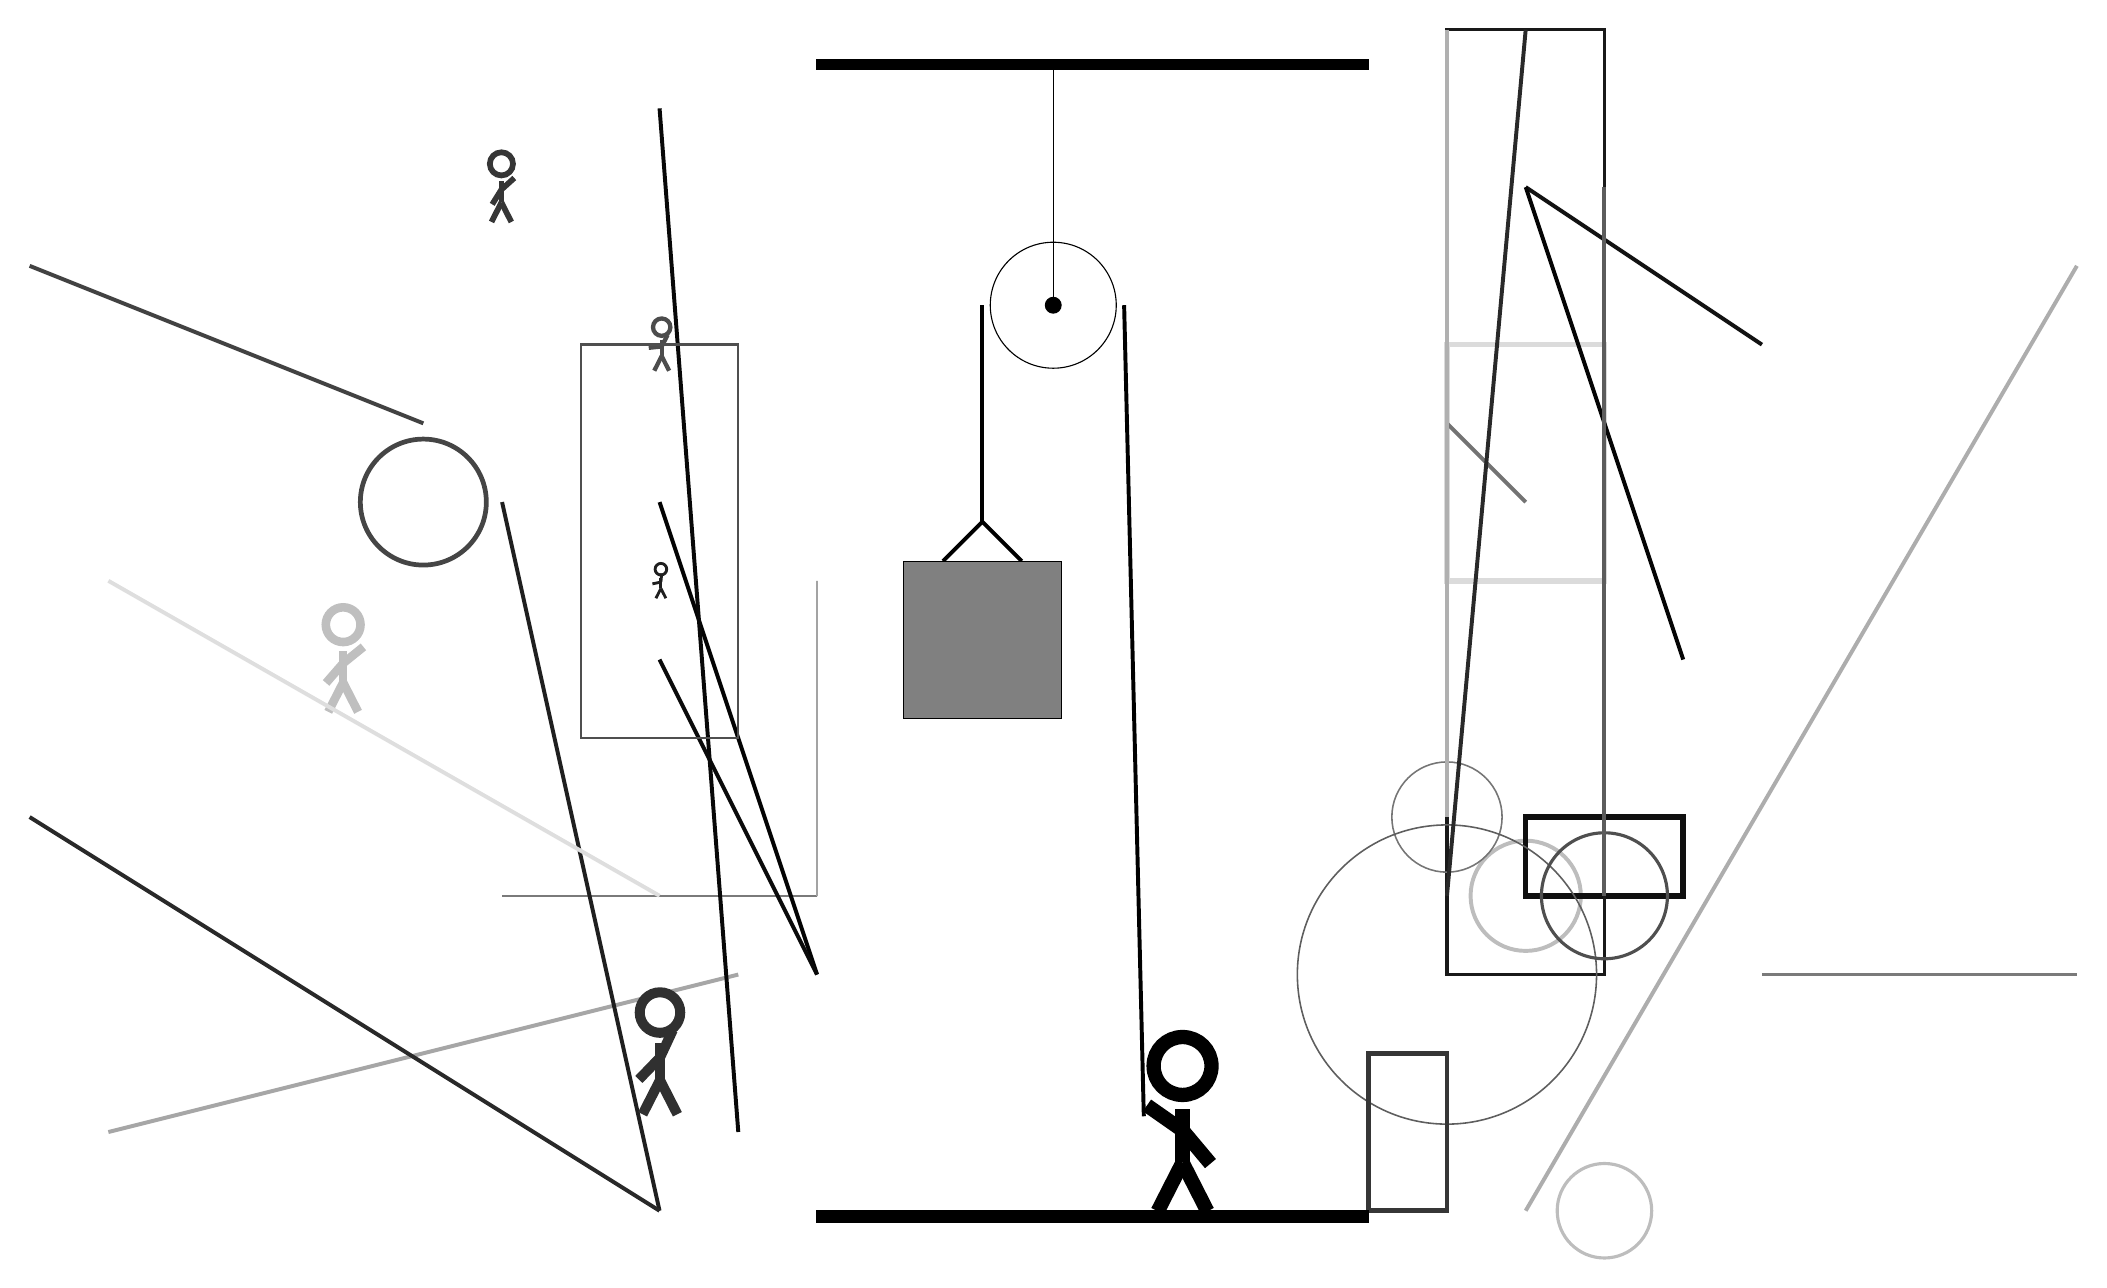
\begin{tikzpicture}
			%%%%% START %%%%%
			
			\draw[fill=black] (-2, 11.5) rectangle (5, 11.625);
			
			\draw (1, 8.5) circle (0.8);
			\draw[fill=black] (1, 8.5) circle (0.1);
			\draw (1, 11.5) -- (1, 8.5);
			
			\draw[line width=0.5mm, color=black!35](-3, 0) -- (-11, -2);
			
			\draw[line width=0.7mm, color=black!14] (6, 8) rectangle (8, 5);
			\draw [line width=0.5mm, color=black!26](7, 1) circle (0.7);
			\draw[line width=0.3mm, color=black!52] (-2, 1) rectangle (-6, 1);
			
			\node[line width=0.5mm, color=black!70] at (-4, 8) {\Strichmaxerl[3][6][63]};
			
			\draw [line width=0.6mm, color=black!73](-7, 6) circle (0.8);
			\draw[line width=0.7mm, color=black!94] (7, 2) rectangle (9, 1);
			
			\draw[line width=0.5mm, color=black!99](-4, 6) -- (-2, 0);
			\draw[line width=0.5mm, color=black!32](7, -3) -- (14, 9);
			\draw[line width=0.5mm, color=black!52](10, 0) -- (14, 0);
			\draw[line width=0.4mm, color=black!90] (6, 12) rectangle (8, 0);
			\draw[line width=0.5mm, color=black!97](-3, -2) -- (-4, 11);
			\draw [line width=0.2mm, color=black!54](6, 2) circle (0.7);
			\draw [line width=0.2mm, color=black!63](6, 0) circle (1.9);
			\draw[line width=0.5mm, color=black!88](-4, -3) -- (-6, 6);
			\draw[line width=0.5mm, color=black!55](7, 6) -- (6, 7);
			
			\draw[line width=0.5mm, color=black!93](10, 8) -- (7, 10);
			\draw [line width=0.4mm, color=black!26](8, -3) circle (0.6);
			\draw [line width=0.4mm, color=black!69](8, 1) circle (0.8);
			
			\draw[line width=0.5mm, color=black!96](-4, 4) -- (-2, 0);
			\draw[line width=0.5mm, color=black!74](-7, 7) -- (-12, 9);
			
			\draw[line width=0.6mm, color=black!79] (5, -3) rectangle (6, -1);
			
			\draw[line width=0.5mm, color=black!84](7, 12) -- (6, 1);
			\draw[line width=0.5mm, color=black!98](7, 10) -- (9, 4);
			\draw[line width=0.5mm, color=black!84](-4, -3) -- (-12, 2);
			
			\draw[line width=0.3mm, color=black!36] (-2, 1) rectangle (-2, 5);
			
			\node[line width=0.4mm, color=black!79] at (-6, 10) {\Strichmaxerl[4][58][42]};
			\draw[line width=0.3mm, color=black!69] (-3, 3) rectangle (-5, 8);
			\node[line width=0.2mm, color=black!25] at (-8, 4) {\Strichmaxerl[6][49][39]};
			\node[line width=0.3mm, color=black!81] at (-4, -1) {\Strichmaxerl[7][46][65]};
			\draw[line width=0.5mm, color=black!13](-4, 1) -- (-11, 5);
			
			\draw[line width=0.5mm, color=black!64](8, 10) -- (8, 1);
			\node[line width=0.4mm, color=black!88] at (-4, 5) {\Strichmaxerl[2][12][85]};
			
			\draw[line width=0.5mm, color=black!31](6, 12) -- (6, 2);
			
			\draw[line width=0.5mm] (-0.4, 5.25) -- (0.1, 5.75) -- (0.6, 5.25);
			\draw[fill=black!50] (-0.9, 5.25) rectangle (1.1, 3.25);
			
			\draw[line width=0.5mm] (0.1, 8.5) -- (0.1, 5.75);
			\centerarc[line width=0.5mm](1, 8.5)(0:180:0.9);
			\draw[line width=0.5mm](1.9, 8.5) -- (2.15, -1.8);
			
			\node at (2.6, -1.9) {\Strichmaxerl[10][-35][-50]};
			
			\draw[fill=black] (-2, -3) rectangle (5, -3.15);
			
			%%%%% END %%%%%
		\end{tikzpicture}
	\end{figure}	
\end{document}